\documentclass[
    a4paper,
    english,
    DIV=16,
    11pt,
    parskip=half,
    listof=totoc,		% lists to toc
    index=totoc,		% index to toc
    bibliography=totoc,	% bibliography to toc
]{scrartcl}
\usepackage[
    pdfhighlight=/O, colorlinks, linkcolor=black, urlcolor=black, citecolor=black,
    breaklinks, bookmarksopen,bookmarksopenlevel=1,linktocpage
] {hyperref} % PDF support with links

\usepackage[english]{babel}
\usepackage[dvips]{graphicx}
\usepackage{amsmath}
\usepackage{enumitem}
\usepackage{float}
\usepackage{microtype}
\usepackage{xcolor}
\usepackage{textcomp}
\usepackage{tikz}
\usepackage{pstricks}
\usepackage{hyperref}
\hypersetup{
    colorlinks,
    citecolor=black,
    filecolor=black,
    linkcolor=blue,
    urlcolor=blue
}
\usepackage{dirtytalk}
\parindent 0pt
\bibliographystyle{alphadin}
\newcommand\todo[1]{\textcolor{red}{#1}}

\title{LaserTag}
\subtitle{An Agent-Based Game Simulation for Testing Intelligent and Goal-Oriented Behavior}
\date{\today\\Version 1.2}
\addtocontents{toc}{\protect\setcounter{tocdepth}{2}}
\setcounter{secnumdepth}{3}

\begin{document}
\maketitle

% ======================================================================

\tableofcontents

% ======================================================================

\clearpage
\section{Introduction}
The LaserTag Framework provides an agent-based game simulation that is inspired by the real-world recreational shooting sport known as laser tag. LaserTag is written in MARS C\#. A number of methods are provided to serve as an interface between agents and the game world (Battleground) and game mechanisms. These methods should be used to play the game as they allow agents to manage their states, move through the Battleground, and interact with other agents upon encountering them.

This documentation will be updated over the next few weeks. Stay tuned for announcements.

\section{Objective} \label{objective}
A team is made up of three agents with the same AI. There are three to four teams per match that compete against each other in a team deathmath game mode. The goal of the game is to score points, and the team with the highest cumulative score at the end of the game wins the match. \textbf{Note:} The goal is not to be the last man/team standing, but to score the highest cumulative number of points across all team members.

% ======================================================================

\section{Project: Setup and Structure}

\subsection{Project Setup}
\label{projsetup}
The project is available in the GitLab repository \href{https://git.haw-hamburg.de/mars/mars-laser-tag-game}{MARS Laser Tag Game}. The directory \textbf{LaserTagBox} contains the game. To use LaserTag, a working installation of JetBrains Rider the MARS C\# plug-in is needed. In Rider, open \textbf{LaserTagBox} to access the game.

\subsection{Project Structure}
\label{projStruc}

The following diagram illustrates the project structure along with properties and methods that are relevant for the AI implementation.

\begin{figure}[H]
    \centering
    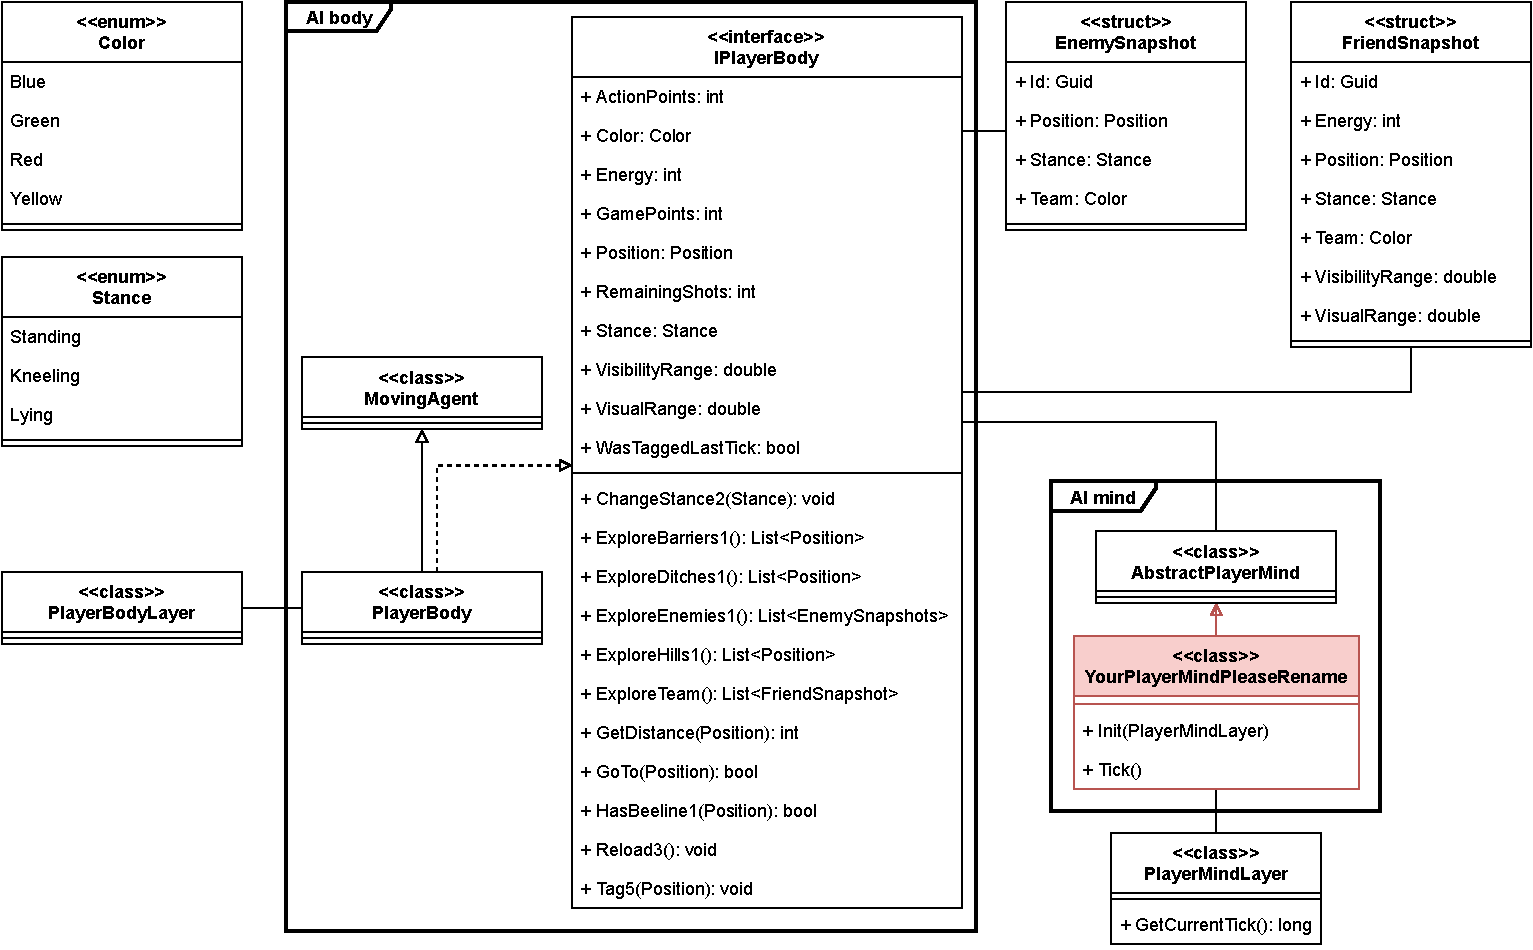
\includegraphics[width=1.0\textwidth, height=0.5\textheight,keepaspectratio]{img/LaserTagStructure.pdf}
    \caption{Diagram illustrating structure of LaserTag in MARS C\#}
    \label{classdiag}
\end{figure}

The implementation of your AI occurs in a class \texttt{YourPlayerMindPleaseRename}, labeled in red in Fig.~\ref{classdiag}, which inherits from the class \texttt{AbstractPlayerMind}. As suggested by the default name, you are welcome to rename the class as you wish. Your AI has a reference to the \texttt{PlayerMindLayer}, from which it may obtain the current simulation tick (\texttt{GetCurrentTick()}), if desired.

The agents' AI has a mental and a physical representation -- mind and body, respectively. The mind controls the body. Through \texttt{AbstractPlayerMind}, the mind obtains a reference to the interface \texttt{IPlayerBody} which has several properties and methods that make up the agent's physical representation. The implementation of these properties and methods is found in the class \texttt{PlayerBody}. Your AI's mind can interact with the interface to guide your AI's body and shape its physical behavior. The class \texttt{MovingAgent} contains auxiliary properties and methods that the body requires to execute some of its functionalities. 

More details regarding the enums, structs, and other parts of the model can be found in subsequent section of the documentation.

\section{Simulation: Setup and Execution}
\label{simSetup}

The game is designed to be played with three or four teams. Use the \texttt{config.json} in the root directory to configure the simulation. This configuration file requires resource files that are contained in the directory \textbf{Resources} -- in particular, a map file and an agent initialization file. The default map is called \texttt{Battleground.csv} and encodes a $50\times 50$ grid cell structure on which the agents can move. The default agent initialization file is called \texttt{player\_positions.csv} and contains the agents' spawn positions on the map.

Simulations can be run via the play button of the IDE.

\section{Visualization: Analyzing Game Outcomes}
A tool with instructions for visualizing simulation results is available in the repository in the directory \textbf{Analysis}. This tool can help you analyze and improve your agents' behavior during the development process. In order for the tool to work, a map file (\texttt{map.csv}) is required in the directory \textbf{Resources/} and a simulation output file (\texttt{PlayerBody.csv}) is required in the directory \textbf{bin/Debug/netcoreapp3.1/}. Once those files are in place, simply double-click \texttt{vis.py} to start the visualizaton tool.

% ======================================================================

\section{Rules} \label{rules}

\subsection{Game Logic}
Below is a list of some of the most important parts of the game's logic:

\begin{itemize}
    \item If an agent's \texttt{Energy} is equal to or below 0, then the agent is taken off the battleground and does not respawn for the rest of the game. The agent's points, however, are maintained and added to the cumulative score of the team at the end of the match.
    \item An agent's \texttt{Energy} regenerates over time. At the end of each tick, an agent's \texttt{Energy} is increased by 1.
\end{itemize}

\subsection{Constraints for AI Developers}
In order to play the game as intended, please adhere to the following rules when implementing your AI:
\begin{enumerate}
    \item Only interact with the interface \texttt{IPlayerBody} to access the agent's physical representation.
    \item If interacting with the \texttt{PlayerMindLayer}, only invoke the \texttt{GetCurrentTick()} method. \item Loops that are known not to terminate after a reasonable time (example: \texttt{while(true)}) are not allowed.
    \item \texttt{PropertyDescription} tags (for loading external information into your agents at runtime) are not allowed.
\end{enumerate}

\section{Agent Properties and Methods} \label{AgentDesc}
The \texttt{IPlayerBody} contains a set of properties and methods that described the agent and define its behavioral capabilities.

\subsection{Properties}

\subsubsection{General properties} \label{genAttr}
\begin{itemize}
    \item \texttt{ActionPoints}: an integer that specifies the number of points the agent has in order to complete actions during the current tick. Each action costs a specific number of \texttt{ActionPoints} (see \ref{methods} for more details). At the end of each tick, \texttt{ActionPoints} is reset to 10.
    \item \texttt{Color}: the agent's color, indicating the agent's team.
    \item \texttt{Energy}: the agent's maximum energy level is 100 and decreases if the agent gets tagged by an opponent. If the energy level is less than or equal to zero, the agent is positioned at its initial spawn position with \texttt{energy = 100}.
    \item \texttt{GamePoints}: the agent's score, which is increased by tagging opponents. Each tag increases the score by 10 points. If a tag causes the opponent's \texttt{energy} to be less than or equal to 0, the tagged agent loses 10 points and an additional 10 points are awarded to the tagger as a bonus.
\end{itemize}

\subsubsection{Movement properties} \label{movAttr}
\begin{itemize}
    \item \texttt{Position}: specifies the agent's current position on the map as a pair of xy-coordinates
    \item \texttt{Stance}: an enum that specifies the agent's current stance. An agent can assume three stances: \texttt{Standing}, \texttt{Kneeling}, and \texttt{Lying}. Each stance affects the property \texttt{VisualRange}, \texttt{VisibilityRange}, and speed at which the agent can move.
\end{itemize}

\subsubsection{Exploration properties} \label{explAttr}
\begin{itemize}
    \item \texttt{VisualRange}: an integer that is set based on the value of \texttt{Stance} and that specifies the agent's current range of sight. The mapping from \texttt{Stance} to \texttt{VisualRange} is as follows:
    \begin{itemize}
        \item \texttt{Standing}$\,\to\,$10
        \item \texttt{Kneeling}$\,\to\,$8
        \item \texttt{Lying}$\,\to\,$5
    \end{itemize}
    \item \texttt{VisibilityRange}: an integer that is set based on the value of \texttt{Stance} and that specifies the maximum distance from which the agent can currently be seen by other agents. The mapping from \texttt{Stance} to \texttt{VisibilityRange} is as follows:
    \begin{itemize}
        \item \texttt{Standing}$\,\to\,$10
        \item \texttt{Kneeling}$\,\to\,$8
        \item \texttt{Lying}$\,\to\,$5
    \end{itemize}
\end{itemize}

\subsubsection{Tagging properties}
\begin{itemize}
    \item \texttt{RemainingShots}: an integer that specifies the agent's currently available opportunities to tag an opponent. If the agent's \texttt{RemainingShots === 0}, then a reload process needs to be initiated.
    \item \texttt{WasTaggedLastTick}: a boolean that specifies if the agent was tagged during the previous tick.
\end{itemize}

These are the properties that may be used to guide the agents through the game. For a full list of properties, please see the source code.

\subsection{Methods} \label{methods}

Below are the methods that an agent's mind may call to guide its body. The digit at the end of the method name indicates the number of \texttt{ActionPoints} required to execute the method. Methods with no digit at the end cost zero \texttt{ActionPoints}.

\subsubsection{Movement Methods}

\begin{itemize}
    \item \texttt{ChangeStance2(Stance)}: this method takes a \texttt{Stance} and allows the calling agent to change between three possible stances: \texttt{Standing}, \texttt{Kneeling}, and \texttt{Lying}. Stance changes affect the values of the agent's \texttt{VisualRange}, \texttt{VisibilityRange}, and movement speed.
    \item \texttt{GoTo(Position) : bool}: this is the main method used for path-finding, movement, and path readjustment. When an agent invokes the method, the method devises a path from the agent's current position to the destination specified by \texttt{Position}. Each subsequent invocation of \texttt{GoTo(Position)} with the same destination will, if possible, move the agent one step closer to the destination until the destination is reached.
    \par
    In order for the agent to change his path before having reached his current destination, \texttt{GoTo(Position)} must be called with a different destination. For example, if the agent is currently moving towards the \texttt{Position} (a, b), this movement process can be interrupted and replaced by a new movement process by calling \texttt{goto((c, d))}, where \texttt{c != a} or \texttt{d != b}.
    \par
    The method returns \texttt{true} when a move was made and \texttt{false} when, for any reason, a move was not made. \textbf{Note:} if \texttt{GoTo(Position)} is called with a destination that refers to a grid cell that is inaccessible (because there is a \texttt{Barrier} on it), then the no path is calculated, no movement is initiated towards the specified destination.
    \par
    For more information on \texttt{goTo(Position)}, please see Sec.~\ref{movement}.
\end{itemize}

\subsubsection{Exploration methods}

\begin{itemize}
    \item \texttt{ExploreBarriers1() : List<Position>}: returns a list of positions of \texttt{Barrier} objects that are in the caller's \texttt{VisualRange} and which the agent can see (\texttt{HasBeeline == true}).
    \item \texttt{ExploreDitches1() : List<Position>}: returns a list of positions of \texttt{Ditch} objects that are in the caller's \texttt{VisualRange} and which the agent can see (\texttt{HasBeeline == true}).
    \item \texttt{ExploreEnemies1(): List<EnemySnapshot>}: this method performs an exploration of opponents in the agent's field of vision and returns a list of \texttt{EnemySnapshot} structs, offering limited information about the identified opponents. 
    \item \texttt{ExploreHills1(): List<Position>}: returns a list of positions of \texttt{Hill} objects that are in the caller's \texttt{VisualRange} and which the agent can see (\texttt{HasBeeline == true}).
    \item \texttt{ExploreTeam(): List<IPlayerBody>}: this method returns a list with references to the calling agent's team, regardless of their location relative to the calling agent.
    \item \texttt{GetDistance(Position) : int}: this method returns the shortest distance (i.e., the number of grid cells) from the calling agent's current position to the specified \texttt{Position}. In order for the distance to be calculable, the grid cell specified by \texttt{Position} must be either visible (based on \texttt{HasBeeline1(Position)}). If the distance to the grid cell specified by \texttt{Position} is not calculable, the method returns \texttt{-1}.
    \item \texttt{HasBeeline1(Position) : bool}: this method may be called by an agent to check if the line of sight between its current position and the grid cell denoted by \texttt{Position} is free from vision-blocking obstacles (i.e., barriers or hills). If it is, the method returns \texttt{true}; otherwise, it returns \texttt{false}.
\end{itemize}

\subsubsection{Tagging methods}
\begin{itemize}
    \item \texttt{Tag5(Position)}: this method takes a \texttt{Position} and attempts to prompts the calling agent to fire a shot onto the grid cell encoded by the position. If an enemy agent is currently located at that position, that agent is tagged.
    \par
    Tagging is implemented as a probability-based process that is influences by both agents' \texttt{Stance} and current positions (ground, hill, or ditch). For example, an agent in the \texttt{Lying} stance has higher accuracy but shorter \texttt{VisualRange}. If an agent is tagged, its \texttt{Energy} is decreased by 10 and the property \texttt{WasTaggedLastTick} is set to \texttt{true}. The tagging agent's \texttt{GamePoints} is increased by 10.
    \par
    For more information on tagging, see \ref{tagging}.
    \item \texttt{Reload3()}: this method prompts the calling agent to reload its tag gun. This is necessary when \texttt{RemainingShots == 0} so that the agent can continue tagging enemies. A successful call to \texttt{Reload3()} refills the calling agent's \texttt{RemainingShots} to 5.
\end{itemize}

% ======================================================================

\section{Model Description} \label{modelDesc}
The model's main components are the Battleground and the properties and methods that serve as an interface for the agents to shape their behavior and decision-making and interact with their environment and with each other.

\subsection{The Arena: Battleground} \label{battleground}
The default Battleground is a $50\times 50$ grid layer. In order to effectively simulate the indoor nature of real-world laser tag, the Battleground is \say{fenced in}. To add texture and complexity to the Battleground and to allow agents to interact with it in meaningful ways, maps may feature barriers, rooms, hills, and ditches (collectively called objects of interest (OOI)).

Below is a bird's eye view of an example of a square-shaped map at the start of the simulation. The following sections describe each of the OOIs. For more information on OOI, see \ref{vision}, \ref{tagging}, and \ref{ooi}.

\begin{figure}[H]
    \centering
    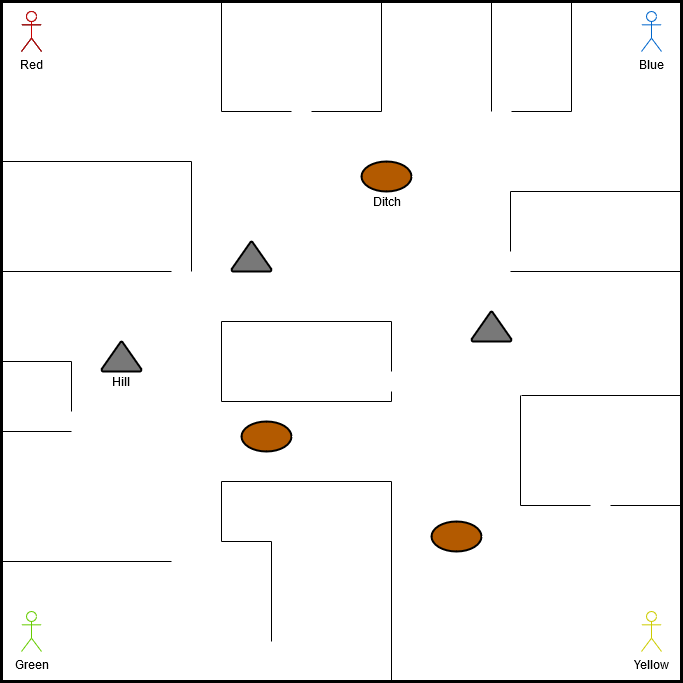
\includegraphics[width=0.5\textwidth, height=0.5\textheight,keepaspectratio]{img/ExampleGameWorldAtSimStart.png}
    \caption{Example of square-shaped map (\texttt{Battleground}) at simulation start (not drawn to scale)}
    \label{battleEx}
\end{figure}

\subsubsection{Structures}
There are a few structural elements in the \texttt{Battleground} that agents can interact with by calling one of the \texttt{Explore*} methods (except \texttt{ExploreTeam} and \texttt{ExploreEnemies1}. Below is a diagram showing the inheritance hierarchy of the structures. Each exploration costs one \texttt{ActionPoint}.

\begin{figure}[H]
    \centering
    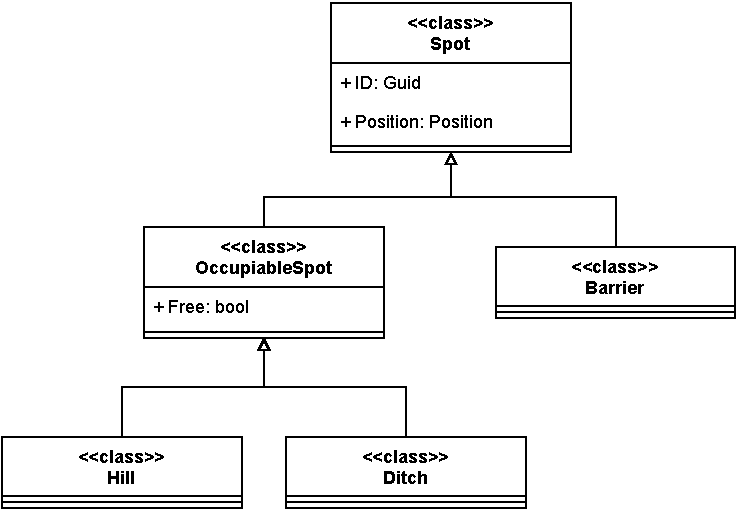
\includegraphics[width=0.5\textwidth, height=0.5\textheight,keepaspectratio]{img/lasertag-env-comps.pdf}
    \caption{Structures}
    \label{structures}
\end{figure}

\paragraph{Barrier}
A \texttt{Barrier} is a structure that cannot be occupied, that acts as an impermeable obstacle to agents, and that disrupts an agent's vision. \texttt{Barrier} instances can be explored by calling \texttt{ExploreBarrier1}.

\paragraph{Hill} \label{hillDesc}
A \texttt{Hill} is a structure that can be occupied. While an agent occupies a \texttt{Hill}, the agent's \texttt{VisualRange} and \texttt{Visibility} are increased. The probability of the agent getting tagged also increases. Occpying a \texttt{Hill} might be a useful team tactic: An agent on a \texttt{Hill} can spot for another agent who is on the ground. \texttt{Hill} instances can be explored by calling \texttt{ExploreHill1}.

\paragraph{Ditch} \label{ditchDesc}
A \texttt{Ditch} is a structure that can be occupied. While an agent occupies a \texttt{Ditch}, the agent's \texttt{VisualRange} and \texttt{Visibility} are decreased. The probability of the agent getting tagged also decreases. Occpying a \texttt{Ditch} might be a useful for ambushing enemies. \texttt{Ditch} instances can be explored by calling \texttt{ExploreDitch1}.

\paragraph{Room}
A room is a section of the grid layer that is enclosed by barriers, leaving only one or more small gaps to enter and exit the enclosed section.

\subsection{Game Mechanics} \label{gameMechs}
This section outlines some of the built-in logic, mechanisms, and rules of LaserTag to help you devise intelligent and feasible strategies for your agents.

\subsubsection{Vision} \label{vision}
The game features a vision system that depends on a number of variables and circumstances. The following example aims to illustrate the process. Agent X calls \texttt{ExploreEnemies1()} and hopes to see agent Y. X's ability to see Y may be influenced by each of the following conditions:
    \begin{enumerate}
        \item the relation between \texttt{distance(X, Y)} and X's \texttt{VisualRange}.
        \item the relation between \texttt{Distance(X, Y)} and Y's \texttt{VisibilityRange}.
        \item whether X or Y is currently located on a \texttt{Hill}.
        \item whether X or Y is currently located in a \texttt{Ditch}.
        \item whether the line of sight between X and Y is obstructed by a barrier or hill.
    \end{enumerate}
    Let us examine each condition in turn:
    \begin{enumerate}
        \item If the distance between X and Y is less than or equal to X's \texttt{VisualRange}, then X may be able to see Y.
        \item If the distance between X and Y is less than or equal to Y's \texttt{VisibilityRange}, then X may be able to see Y. Y's \texttt{VisibilityRange} is irrelevant for when X stands either on a \texttt{Hill} or in a \texttt{Ditch}.
        \item A barrier or \texttt{Hill} can block an agent's line of sight. If there is nothing blocking X's line of sight to Y, then X may be able to see Y. (For more information on line-of-sight computation, feel free to check out \href{http://tech-algorithm.com/articles/drawing-line-using-bresenham-algorithm/}{Bresenham's Line Algorithm} which is implemented in LaserTag to determine if any of the grid cells along the line of sight between two agents holds an vision-blocking object (a barrier or \texttt{Hill}).
        \item If X is located on a \texttt{Hill}, then his \texttt{VisualRange} is increased, making it possible for him to see Y from a farther distance. Likewise, if Y is located on a hill, then his \texttt{VisibilityRange} is increased, making it easier for X to see him.
        \item If X is located in a \texttt{Ditch}, then his \texttt{VisualRange} is decreased, which requires Y to be closer to X in order for X to be able to see Y. Likewise, if Y is located in a \texttt{Ditch}, then his \texttt{VisibilityRange} is decreased, requiring X to be closer to Y in order for X to be able to see Y.
    \end{enumerate}
    Conditions 1, 2, and 3 must be met in order for X to be able to see Y. Conditions 4 and 5 merely describe how standing on a \texttt{Hill} or in a \texttt{Ditch} might affect the vision process.
    
\subsubsection{Movement} \label{movement}
Agents move along the grid via a modified version of the \href{http://idm-lab.org/bib/abstracts/papers/aaai02b.pdf}{D* Lite Algorithm}. The algorithm computes an initial (usually close-to-optimal or optimal) route from an agent's current position to the desired destination. Once the route has been calculated, the algorithm guides the agent towards the goal at a rate dependent on the agent's \texttt{Stance} and movement capabilities. The algorithm performs route adjustments and recalculations only if an obstacle intersects the agent's path that was not present during the initial route computation. This makes the algorithm highly efficient and perform at a better time complexity than more common path-finding algorithms such as A*.

\subsubsection{Tagging} \label{tagging}
Tagging is the core game mechanic that drives LaserTag. In an attempt to simulate real-world tag-and-get-tagged interactions between laser tag players, the method \texttt{Tag5(Position)} relies on probability and randomization to create a balance between successful and unsuccessful tag attempts. If agent X attempts to tag agent Y, the outcome depends on the following factors:
    \begin{enumerate}
        \item X's \texttt{Stance}
        \item Y's \texttt{Stance}
        \item whether Y is currently positioned on a regular grid cell, a hill, or a ditch
        \item a dose of luck
    \end{enumerate}
    Let us examine each factor in turn:
    \begin{enumerate}
        \item If X's \texttt{Stance == Lying}, then he is most likely to tag Y. If X's \texttt{Stance == Standing}, then he is least likely to tag Y.
        \item If Y's \texttt{Stance == Standing}, then X is most likely to tag him. If Y's \texttt{Stance == Lying}, then X is least likely to tag him.
        \item If Y is located on a \texttt{Hill}, then his \texttt{Stance} cannot lower the likelihood of him being tagged. This is because being on a \texttt{Hill} leads to more exposure than being on the ground or in a \texttt{Ditch}. Conversely, if Y is located in a \texttt{Ditch}, then his \texttt{Stance} does not increase his likelihood of being tagged. This is because a being in a \texttt{Ditch} provides increased cover regardless of the agent's \texttt{Stance}.
        \item Even if factors 1-3 are in Y's favor, there is still a chance that X tags Y. On the other hand, even if factors 1-3 are in X's favor, there is still a chance that he might miss Y and not tag him. This is due to the element of randomization added to the tagging mechanism.
    \end{enumerate}

\subsubsection{OOI} \label{ooi}
The Battleground features \texttt{Hills} and \texttt{Ditches} as objects for agents to interact with and, under certain circumstances, gain an advantage over their opponents. A \texttt{Hill} or \texttt{Ditch} can be occupied by only one agent at a time. Being on a \texttt{Hill} increases an agent's \texttt{VisualRange} and \texttt{VisibilityRange} by five each. Being in a \texttt{Ditch} lowers an agent's \texttt{VisualRange} and  \texttt{VisibilityRange} by three each. See \ref{vision} and \ref{tagging} as well as \ref{hillDesc} and \ref{ditchDesc} for more information.

\end{document}
